\myparagraph{Purpose}
Any user can manage his personal profile both from \textit{Data4Help} web site and from \textit{AutomatedSOS} or \textit{Track4Run} applications. In particular:
\begin{itemize}
  \item The user can change some of his personal informations: his/her city of residence, his/her address and his/her occupation.
  \item The user can see the data acquired on him/her until this moment;
  \item The user can see the past received requests about seeing his/her personal data;
  \item The user can see the pending received requests about seeing his/her personal data and accept/refuse them;
  \item The user can change his/her password;
  \item The user can change the device associated to his/her profile (only from \textit{AutomatedSOS} or \textit{Track4Run} applications);
  \item The user can delete his/her profile.
\end{itemize}

\myparagraph{Scenario 1}
Chiara has just finished her studies and has just found a new job, so she wants to update the occupation field on her profile. She opens \textit{Data4Help} web site from her personal computer, she logs in and goes in her "\textit{Edit profile}" area. The system gives her the possibility to change either her city of residence or her occupation, she changes her occupation from student to emplyed and she clicks on the "\textit{Submit changes}" button.

\myparagraph{Scenario 2}
Matteo has just finished the registration process, but he doesn't like the password he was given by the system and he wants to change it. He opens \textit{AutomatedSOS} application on his smartphone, logs in and accesses to his "\textit{Edit profile}" area. Now he clicks on the "\textit{Change password}" button and inserts the old password and the new password twice as required by the system. Finally he clicks on the "\textit{Submit changes}" button.

\myparagraph{Scenario 3}
Aldo moved to USA and so he decides to delete his profile on \textit{Track4Run} because he was used to use it to organize amateur runs with his friends, but now he won't be able to do it anymore. He opens \textit{Track4Run} application on his smartphone, logs in and accesses to his "\textit{Edit profile}" area. Now he clicks on the "\textit{Delete profile}" button and confirms his choice. The system removes all Aldo's information from the database.

\myparagraph{Scenario 4}
Franco has just received a new smartwatch for his birthday and so he wants to change the device associated to his \textit{Data4Help} profile. He opens \textit{Track4Run} application on his smartphone, logs in and accesses to his "\textit{Edit profile}" area. Then he clicks on "\textit{Change device}" button and turns on the bluetooth of the new smartwatch and of his smartphone. He selects the new smartwatch among those that appears on the smartphone's screen and clicks on "\textit{Done}" button. Now he can use his new smartwatch;

\myparagraph{Use Case}
The \textit{Profile Visualization} use case is analyzed in Table \ref{table:profileVisualizationTable}. \\
The \textit{Modify Personal Information} use case is analyzed in Table \ref{table:modifyPersonalInformationTable}. \\
The \textit{Change Password} use case is analyzed in Table \ref{table:changePassowrdTable}. \\
The \textit{Change Device} use case is analyzed in Table \ref{table:changeDeviceTable}. \\
The \textit{Delete Profile} use case is analyzed in Table \ref{table:deleteProfileTable} \\

\myparagraph{Activity Diagram}
The \textit{Profile Visualization} activity diagram is shown in Figure \ref{img:profileVisualizationActivityDiagram}. \\
The \textit{Modify Personal Informations} activity diagram is shown in Figure \ref{img:modifyPersonalInformationsActivityDiagram}. \\
The \textit{Change Password} activity diagram is shown in Figure \ref{img:changePasswordActivityDiagram}. \\
The \textit{Change Device} activity diagram is similar to the one shown in Figure \ref{img:firstIndividualLoginActivityDiagram}. \\
The \textit{Delete Profile} activity diagram is shown in Figure \ref{img:deleteProfileActivityDiagram}.

\myparagraph{Mockup}
The \textit{Manage Profile} mocukp is shown in Figure \ref{img:manageProfileMockup}.

\myparagraph{Functional requirements}
\begin{enumerate}
  \item The system must let the user view his/her personal profile at anytime;
  \item The system must let the user upload/change his/her personal information at anytime;
  \item The system must let the user change his password only if the old one has been inserted correctly;
  \item The system must not let the user change his password if the new one has not been inserted correctly twice;
  \item The system must let the user change the device connected to his/her profile at anytime;
  \item The system must let the user delete his/her profile at anytime;
  \item The system must require to confirm a deleting request;
  \item The system must not delete a profile if the choice isn't confirmed by the user;
  \item The system must let the user leave the editing profile process at anytime;
  \item The system must delete all user's personal information from its database when the user decides to delete his/her profile;
  \item The system must let the user accept/refuse an individual data request at anytime.
\end{enumerate}

\begin{center}
\begin{table}[H]
\begin{tabular}{ | l | p{0.75\linewidth} | }
  \hline
    Actor & \textbf{User} \\ \hline
    Goal & \textbf{[G.3]} \\ \hline
    Input Condition & A \textbf{User} wants to view his personal profile\\ \hline
    Event Flow & \begin{minipage}[t]{0.7\textwidth}
      \begin{enumerate}
        \item The \textbf{User} opens \textit{Data4Help} web site or \textit{AutomatedSOS} or \textit{Track4Run} applications;
        \item The \textbf{User} logs in;
        \item The \textbf{User} accesses to his personal area;
        \item The system shows to the \textbf{User} his/her "\textit{Edit profile}" area and the buttons to move to "\textit{Acquired Data}" area, "\textit{Past Requests}" area and "\textit{Pending Requests}" area.
      \end{enumerate}
    \smallskip
  \end{minipage} \\ \hline
  Output Condition & The \textbf{User} views his/her personal profile\\ \hline
  Exceptions & None \\ \hline
\end{tabular}
\caption{\textit{Profile Visualization} use case}
\label{table:profileVisualizationTable}
\end{table}
\end{center}

\begin{figure}[H]
\begin{center}
  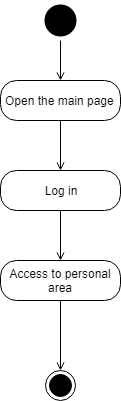
\includegraphics{img/activity/ProfileVisualization.png}
  \hspace{0.05\linewidth}
  \centering
  \caption{\textit{Profile Visualization} activity diagram from user's point of view}
  \label{img:profileVisualizationActivityDiagram}
\end{center}
\end{figure}

\begin{center}
\begin{table}[H]
\begin{tabular}{ | l | p{0.75\linewidth} | }
  \hline
    Actor & \textbf{User} \\ \hline
    Goal & \textbf{[G.3]} \\ \hline
    Input Condition & A \textbf{User} wants to modify his/her personal information\\ \hline
    Event Flow & \begin{minipage}[t]{0.7\textwidth}
      \begin{enumerate}
        \item The \textbf{User} opens \textit{Data4Help} web site or \textit{AutomatedSOS} or \textit{Track4Run} applications;
        \item The \textbf{User} logs in;
        \item The \textbf{User} accesses to his/her personal area;
        \item The \textbf{User} goes in "\textit{Edit profile}" area;
        \item The system shows the \textbf{User} the modifiable information;
        \item The \textbf{User} modifies what he/she wants;
        \item The \textbf{User} clicks on the "\textit{Submit changes}" button;
      \end{enumerate}
    \smallskip
  \end{minipage} \\ \hline
  Output Condition & The \textbf{User}'s information are modified\\ \hline
  Exceptions & \begin{minipage}[t]{0.7\textwidth}
    \begin{itemize}
      \smallskip
      \item If the \textbf{User} decides to leave the editing process this one is aborted.
    \end{itemize}
    \smallskip
  \end{minipage}  \\ \hline
\end{tabular}
\caption{\textit{Modify Personal Information} use case}
\label{table:modifyPersonalInformationTable}
\end{table}
\end{center}

\begin{figure}[H]
\begin{center}
  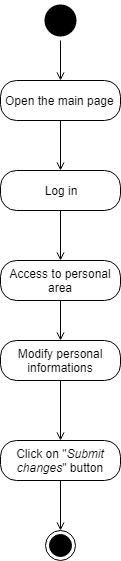
\includegraphics[height=0.6\paperheight]{img/activity/ModifyPersonalInformations.png}
  \hspace{0.05\linewidth}
  \centering
  \caption{\textit{Modify Personal Information} activity diagram from user's point of view}
  \label{img:modifyPersonalInformationsActivityDiagram}
\end{center}
\end{figure}

\begin{center}
\begin{table}[H]
\begin{tabular}{ | l | p{0.75\linewidth} | }
  \hline
    Actor & \textbf{User} \\ \hline
    Goal & \textbf{[G.3]} \\ \hline
    Input Condition & A \textbf{User} wants to change his password\\ \hline
    Event Flow & \begin{minipage}[t]{0.7\textwidth}
      \begin{enumerate}
        \item The \textbf{User} opens \textit{Data4Help} web site or \textit{AutomatedSOS} or \textit{Track4Run} applications;
        \item The \textbf{User} logs in;
        \item The \textbf{User} accesses to his personal area;
        \item The \textbf{User} goes in "\textit{Edit profile}" area;
        \item The \textbf{User} clicks on the "\textit{Change password}" button;
        \item The system shows the \textbf{User} the fields in which he/she has to insert the old and the new password;
        \item The \textbf{User} inserts the old password;
        \item The \textbf{User} inserts the new password twice;
        \item The \textbf{User} clicks on the "\textit{Submit changes}" button;
      \end{enumerate}
    \smallskip
  \end{minipage} \\ \hline
  Output Condition & The \textbf{User}'s password is modified\\ \hline
  Exceptions & \begin{minipage}[t]{0.7\textwidth}
    \begin{itemize}
      \smallskip
      \item If functional requirement 3 is not satisfied the system goes back to step 7;
      \item If functional requirement 4 is not satisfied the system goes back to step 8;
      \item If the \textbf{User} decides to leave the editing process this one is aborted.
    \end{itemize}
    \smallskip
  \end{minipage}  \\ \hline
\end{tabular}
\caption{\textit{Change Password} use case}
\label{table:changePassowrdTable}
\end{table}
\end{center}

\begin{figure}[H]
\begin{center}
  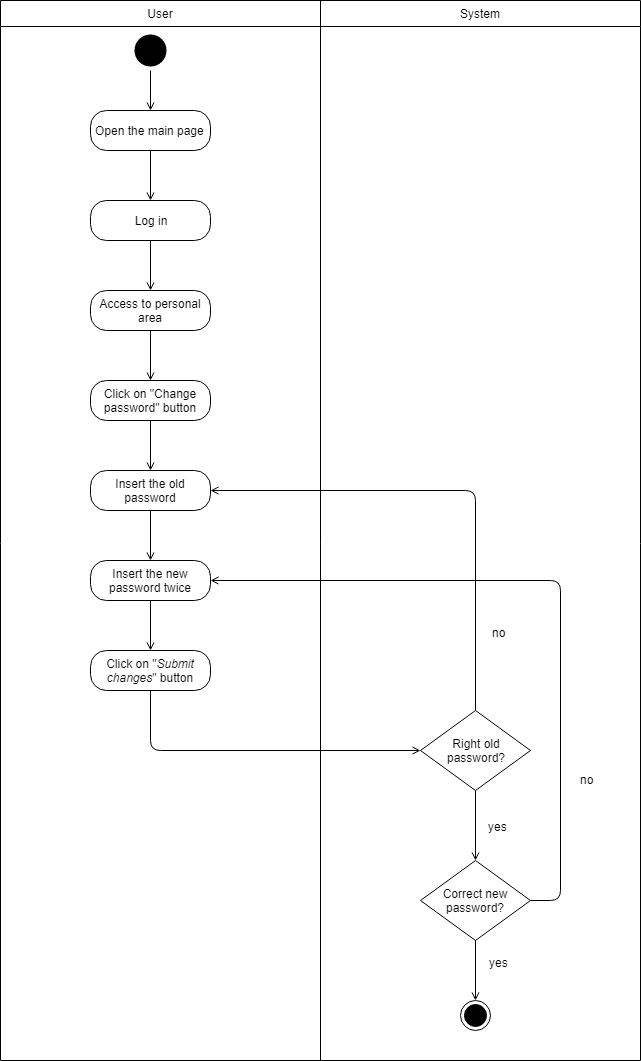
\includegraphics[height=0.6\paperheight]{img/activity/ChangePassword.png}
  \hspace{0.05\linewidth}
  \centering
  \caption{\textit{Change Password} activity diagram}
  \label{img:changePasswordActivityDiagram}
\end{center}
\end{figure}

\begin{center}
\begin{table}[H]
\begin{tabular}{ | l | p{0.75\linewidth} | }
  \hline
    Actor & \textbf{User} \\ \hline
    Goal & \textbf{[G.3]} \\ \hline
    Input Condition & A \textbf{User} wants to change the associated device\\ \hline
    Event Flow & \begin{minipage}[t]{0.7\textwidth}
      \begin{enumerate}
        \item The \textbf{User} opens \textit{AutomatedSOS} or \textit{Track4Run} applications;
        \item The \textbf{User} logs in;
        \item The \textbf{User} accesses to his personal area;
        \item The \textbf{User} goes in "\textit{Edit profile}" area;
        \item The \textbf{User} clicks on the "\textit{Change device}" button;
        \item The system asks the \textbf{User} to turn on the bluetooth of the smartwatch and of the smartphone;
        \item The \textbf{User} turns on the bluethooth;
        \item The system shows on the smartphone display the associable devices that it finds with the bluetooth connection;
        \item The \textbf{User} selects the device he wants to associate.
        \item The \textbf{User} clicks on "\textit{Done}" button.
      \end{enumerate}
    \smallskip
  \end{minipage} \\ \hline
  Output Condition & The new device is correctly connected to the \textbf{User}'s smartphone \\ \hline
  Exceptions & \begin{minipage}[t]{0.7\textwidth}
    \begin{itemize}
      \smallskip
      \item If the \textbf{User} decides to leave the changing device process this one is aborted.
    \end{itemize}
    \smallskip
  \end{minipage}  \\ \hline
\end{tabular}
\caption{\textit{Change Device} use case}
\label{table:changeDeviceTable}
\end{table}
\end{center}

\begin{center}
\begin{table}[H]
\begin{tabular}{ | l | p{0.75\linewidth} | }
  \hline
    Actor & \textbf{User} \\ \hline
    Goal & \textbf{[G.3]} \\ \hline
    Input Condition & A \textbf{User} wants to delete his/her profile\\ \hline
    Event Flow & \begin{minipage}[t]{0.7\textwidth}
      \begin{enumerate}
        \item The \textbf{User} opens \textit{Data4Help} web site or \textit{AutomatedSOS} or \textit{Track4Run} applications;
        \item The \textbf{User} logs in;
        \item The \textbf{User} accesses to his personal area;
        \item The \textbf{User} goes in "\textit{Edit profile}" area;
        \item The \textbf{User} clicks on the "\textit{Delete profile}" button;
        \item The \textbf{User} confirms his/her choice;
      \end{enumerate}
    \smallskip
  \end{minipage} \\ \hline
  Output Condition & The \textbf{User}'s  profile is deleted\\ \hline
  Exceptions & \begin{minipage}[t]{0.7\textwidth}
    \begin{itemize}
      \smallskip
      \item If functional requirement 8 is not satisfied the deleting process is aborted;
      \item If the \textbf{User} decides to leave the deleting process this one is aborted.
    \end{itemize}
    \smallskip
  \end{minipage}  \\ \hline
\end{tabular}
\caption{\textit{Delete Profile} use case}
\label{table:deleteProfileTable}
\end{table}
\end{center}

\begin{figure}[H]
\begin{center}
  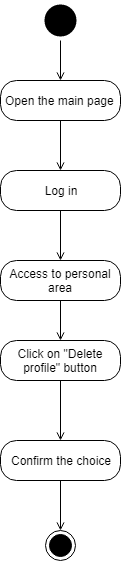
\includegraphics[height=0.6\paperheight]{img/activity/DeleteProfile.png}
  \hspace{0.05\linewidth}
  \centering
  \caption{\textit{Delete Profile} activity diagram from user's point of view}
  \label{img:deleteProfileActivityDiagram}
\end{center}
\end{figure}

\begin{figure}[H]
\begin{center}
  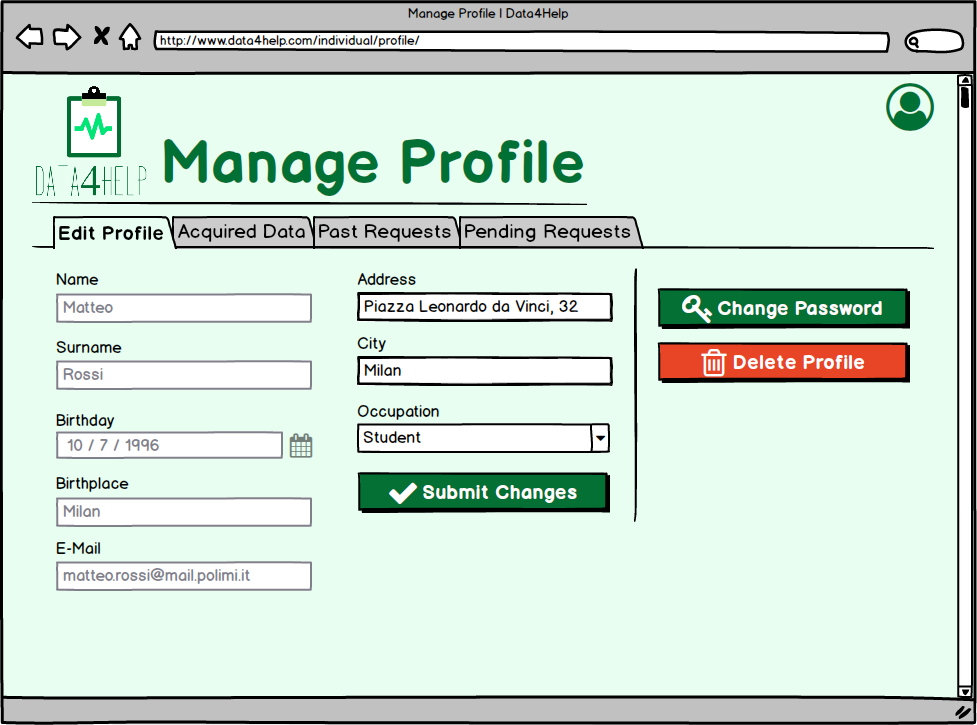
\includegraphics[width=\textwidth]{img/mockup/Manage_Profile.png}
  \hspace{0.05\linewidth}
  \centering
  \caption{\textit{Manage Profile} mockup}
  \label{img:manageProfileMockup}
\end{center}
\end{figure}
